\documentclass{../../sheet}
\renewcommand{\logopath}{../../logos/}

\title{PSE Vorkurs Tag 5}

\begin{document}
\maketitle
Heute Abend UNO!


\aufgabe{Feedback}
Bitte füllt den Feedbackbogen aus, damit wir den Vorkurs für die nächsten Jahre verbessern können. Der Bogen ist anonym und dauert diesmal ein bisschen länger. \newline Ihr findet ihn unter: \url{https://forms.gle/HhisY91RZc8eDkPy5}
\aufgabe{Musterlösungen}
\href{https://fius.de/wp-content/uploads/2025/10/Day4Musterloesung.zip}{Tag 4 Lösungen}

\aufgabe{Präsentations-Cheatsheet}
\textbf{Map Funktionen:}
\begin{table}[h]
    \centering
    \rowcolors{2}{tablerow}{white}
    \begin{tabular}{l l}
        \rowcolor{tablehead}
        \textbf{Methode}        & \textbf{Beschreibung}                    \\
        \texttt{put(k, v)}      & Fügt einen neuen Schlüssel-Wert-Paar ein \\
        \texttt{get(k)}         & Gibt den Wert zu einem Schlüssel zurück  \\
        \texttt{remove(k)}      & Entfernt einen Eintrag                   \\
        \texttt{containsKey(k)} & Prüft, ob Schlüssel existiert            \\
        \texttt{keySet()}       & Gibt alle Schlüssel zurück               \\
        \texttt{values()}       & Gibt alle Werte zurück                   \\
        \texttt{size()}         & Gibt die Anzahl der Einträge zurück      \\
    \end{tabular}
\end{table}

\textbf{Map-Syntax:}

\begin{minted}[linenos=false]{java}
import java.util.HashMap;

HashMap<String, Integer> studis = new HashMap<>();
studis.put("Melanie", 1976370);
studis.put("Paul", 1249609);

System.out.println(studis.get("Melanie"));
	\end{minted}


\newpage
\aufgabe{Aufgabe 1: Maps}
Maps verbinden ein Schlüsselelement mit einem Wert. Diese können auch unterschiedliche Datentypen haben. Ein Telefonbuch könnte beispielsweise als Map dargestellt werden um Namen mit Telefonnummern zu verbinden:
\begin{minted}[linenos=false]{java}
Map<String, Long> telefonbuch = new HashMap<String, Long>();
//erstes Parameter ist der Schlüssel, zweites ist der Wert
telefonbuch.put("Paul Griller", 1374927394);
telefonbuch.put("Melanie Barbecue", 9257632984);
\end{minted}

\begin{enumerate}
    \item Schreibe eine Funktion die einen Dictionary entgegennimmt und alle Schlüssel und die dazugehörigen Werte ausgibt:

          \begin{ausgabe}
              Paul Griller: 1374927394, Melanie Barbecue: 9257632984
          \end{ausgabe}

    \item Schreibe eine Funktion die einen String entgegennimmt und in einem Dictionary speichert, wie oft jeder Buchstabe darin vorkommt.

          \begin{ausgabe}
              grimmige griller grillen glühend gern grobe grillgemüse-spieße.
          \end{ausgabe}
          wird mithilfe der Ausgabe-Funktion aus Aufgabe 1.1 zu:
          \begin{ausgabe}
              g: 9, r: 7, i: 6, m: 3, e: 10,  : 6, l: 7, n: 3, ü: 2, h: 1, d: 1, o: 1, b: 1, s: 2, -: 1, p: 1, ß: 1, .: 1
          \end{ausgabe}

          Hinweis: Verwende die \texttt{split("")} Funktion auf einem String um ihn in ein Zeichenarray umzuwanden. Mehr dazu findest du hier: \url{https://docs.oracle.com/javase/8/docs/api/java/lang/String.html#split-java.lang.String-}.

    \item Erweitere deine Funktion, sodass sie zusätzlich zum String einen Integer \texttt{length} entgegennimmt und statt einzelne Buchstaben, jetzt Buchstabenfolgen der Länge \texttt{length} zählt.

          \begin{ausgabe}
              grimmige griller grillen glühend gern grobe grillgemüse-spieße.
          \end{ausgabe}
          wird bei \texttt{length = 3} zu:
          \begin{ausgabe}
              gri: 4, rim: 1, imm: 1, mmi: 1, mig: 1, ige: 1, ge : 1, e g: 2,  gr: 4, ril: 3, ill: 3, lle: 2, ler: 1, er : 1, r g: 1, len: 1, en : 1, n g: 2,  gl: 1, glü: 1, lüh: 1, ühe: 1, hen: 1, end: 1, nd : 1, d g: 1,  ge: 1, ger: 1, ern: 1, rn : 1, gro: 1, rob: 1, obe: 1, be : 1, llg: 1, lge: 1, gem: 1, emü: 1, müs: 1, üse: 1, se-: 1, e-s: 1, -sp: 1, spi: 1, pie: 1, ieß: 1, eße: 1, ße.: 1
          \end{ausgabe}

\end{enumerate}

\newpage
\aufgabe{Aufgabe 2: Datenstrukturen selber erstellen}
In Java kann jederzeit eine neue Datenstruktur gebaut werden, die dann auch an die Eigenheiten der Problemstellung angepasst sein kann. \\
Ihr habt ja sicher schon gemerkt, das Arrays etwas sperrig zu nutzen sind, da deren Größe komplett statisch ist. Im Folgenden bauen wir eine Listen-Datenstruktur welche dieses Problem löst. Sie soll aus einzelnen Knotenobjekten bestehen, die dann untereinander verbunden werden. \\
\\
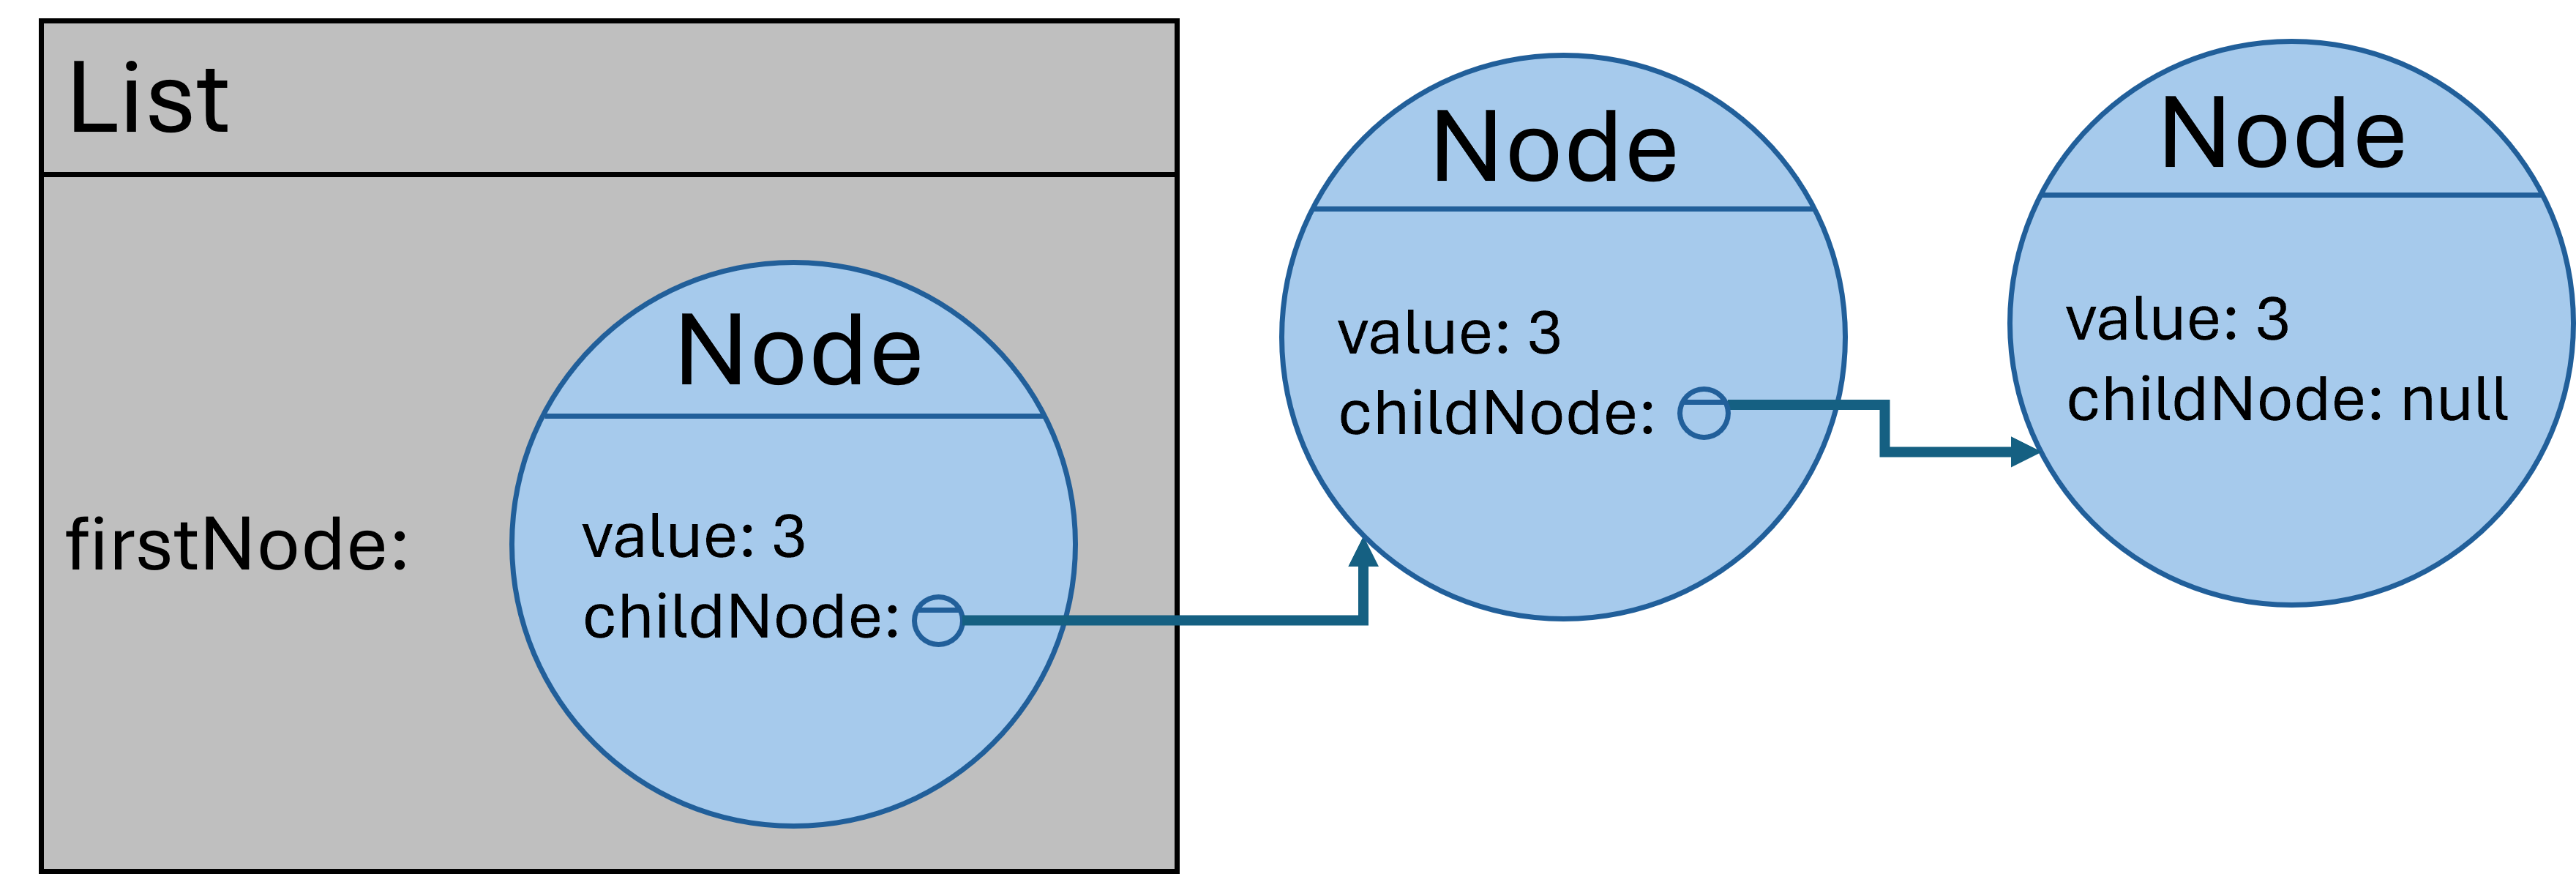
\includegraphics[width=\linewidth]{img/linkedlist.png}

\begin{enumerate}
    \item Erstelle eine Knotenklasse namens \texttt{Node}. Jede Knotenklasse soll einen Wert \texttt{value} vom Typ \texttt{int}, sowie einen Folgeknoten \texttt{nextNode} vom Typ \texttt{Node} als Attribute haben. Erstelle einen sinnvollen Konstruktor.
    \item Erstelle jetzt die Listenklasse. Jede \texttt{List} hat einen Startknoten \texttt{startNode}. Programmiere wieder einen sinnvollen Konstruktor.
    \item Noch besteht jede dieser Listen nur aus einem einzelnen Startknoten. Füge um das zu ändern der \texttt{List} Klasse eine \texttt{add(Node newElement)} Funktion hinzu. Sie soll eine neue Node ans Ende der Liste anfügen.
    \item Gib der \texttt{List} Klasse außerdem eine \texttt{remove(Node element)} Funktion. Achte darauf, dass dabei eventuelle Folgeelemente nicht ''Elternlos'' zurückgelassen werden.
    \item Programmiere eine \texttt{printElements()} Funktion, die alle Elemente in der Liste anschaulich in der Konsole ausgibt.
    \item In dieser Aufgabe soll die Summe der Werte unserer Liste berechnet werden. Schreibe dazu eine Funktion in der Klasse Node, die die bisherige Summe entgegennimmt, ihren eigenen Wert hinzuaddiert und sich dann im nächsten Knoten selbst aufruft. Wenn die Methode auf den letzten Knoten in der Liste stößt, soll die berechnete Gesamtsumme zurückgegeben werden. Füge zuletzt der Klasse „List“ eine Funktion hinzu, die die Summenfunktion im ersten Knoten (natürlich mit bisheriger Summe 0) aufruft.
\end{enumerate}

Du hast gerade eine einfache LinkedList programmiert. LinkedLists sind sehr wichtig als Datenstruktur mit Variabler Größe und sie existieren auch in nativem Java: \url{https://docs.oracle.com/javase/8/docs/api/java/util/LinkedList.html}

\newpage
\aufgabe{HIGHPERFORMER-Aufgabe: Bäume}
Bäume sind auch eine wichtige Datenstruktur in Java. Bei einem Baum ist jeder Knoten mit Kindknoten verbunden, welche wiederum mit weiteren Kindknoten verbunden sind. So werden die Daten in einer Art Baumstruktur gespeichert. Binärbäume sind besondere Bäume, bei welchen jeder Knoten maximal zwei Kindknoten haben darf: 
\\
\begin{center}
    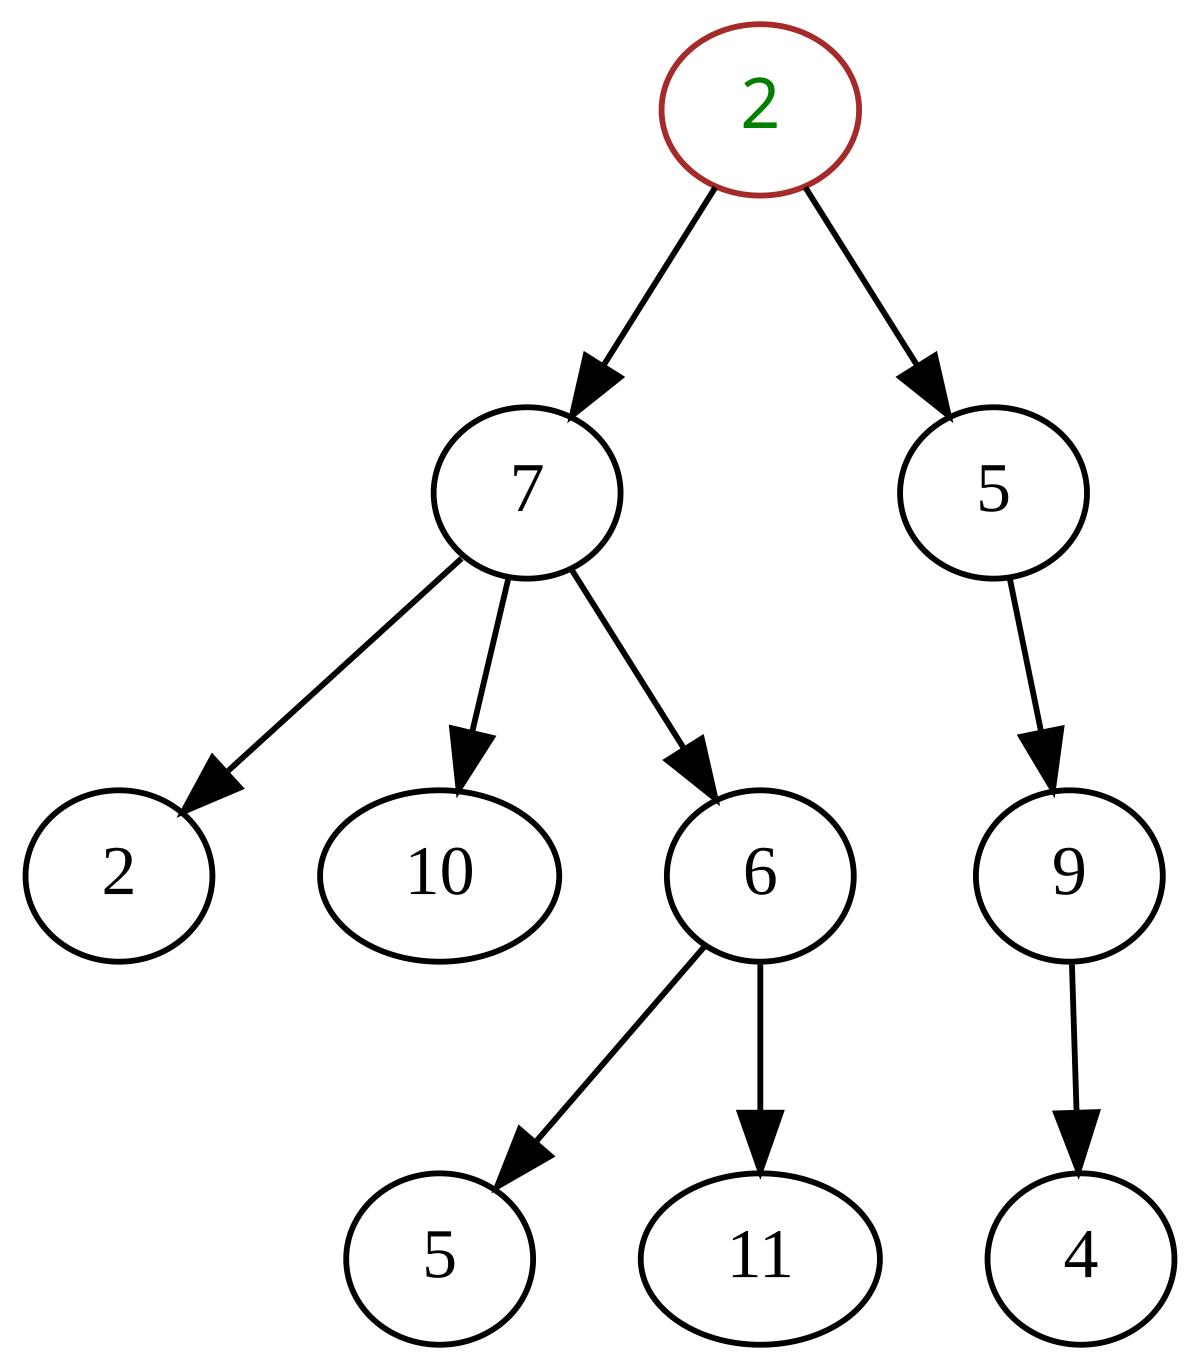
\includegraphics[width=0.5\linewidth]{img/baum.png}
\end{center}

\begin{enumerate}
    \item Erstelle eine \texttt{BinaerBaum}-Klasse, die einen Wurzelknoten besitzt, sowie eine \texttt{Knoten}-Klasse, die einen \texttt{int}-Wert, sowie genau zwei Kindknoten (\texttt{linkesKind} und \texttt{rechtesKind}) speichert. Wenn ein Knoten bspw. kein rechtes Kind hat soll der Wert von \texttt{rechtesKind} gleich \texttt{null} sein. Da jeder Knoten maximal zwei Kinder hat ist der Baum ein sogenannter binärer Baum.
    \item Programmiere eine Funktion in der \texttt{BinaerBaum}-Klasse, die eine neue Zahl in den Baum einfügt. Diese Funktion soll den Baum Knoten für Knoten durchgehen und bei jedem Knoten zufällig zum rechten oder linken Kind ''abbiegen''. Sobald auf ein \texttt{null} gestoßen wird, wird der einzufügende Wert dort mit einem neuen Knoten hinzugefügt.
    \item Programmiere eine Funktion in der \texttt{BinaerBaum}-Klasse, die den Baum anschaulich in der Konsole ausgibt.
    \item Programmiere zwei Funktionen, eine die den Baum eindeutig in eine LinkedList (die aus Aufgabe 2.) umwandelt und eine die dasselbe umgekehrt macht. Überlege dir hierfür eine Möglichkeit wie die Struktur des Baums in der Liste abgebildet werden kann.\\
    Hinweis: Du kannst deine Funktionen Testen indem du einen Baum zu einer LinkedList umwandeln lässt und dann mit der anderen Funktion zurück zu einem Baum umwandelst und dann prüfst ob die Struktur erhalten geblieben ist.
    \item Programmiere eine Funktion \texttt{maxPathSum} in der \texttt{BinaerBaum}-Klasse, die einen \texttt{BinaerBaum} entgegennimmt und die maximale Pfadsumme für diesen Baum berechnet. Es werden alle Knoten entlang eines Pfades von oben nach unten addiert und die höchste Summe soll zurückgegeben werden. Bei dem obigen Beispielbaum wäre die maximale Pfadsumme 26 für den Pfad \texttt{2 - 7 - 6 - 11} . 
\end{enumerate}
\newpage
\aufgabe{Feedback}
Bitte füllt den Feedbackbogen aus, damit wir den Vorkurs für die nächsten Jahre verbessern können. Der Bogen ist anonym und dauert diesmal ein bisschen länger. \newline Ihr findet ihn unter: \url{https://forms.gle/HhisY91RZc8eDkPy5}

\end{document}